\documentclass[border=8pt]{article}
\usepackage{tikz}
\usepackage{geometry}
\geometry{margin=0.5cm}
\usetikzlibrary{positioning}
\usetikzlibrary{quotes,arrows.meta}
\usetikzlibrary{shapes.geometric}

% Define colors
\def\ConvColor{rgb:yellow,5;red,2.5;white,5}
\def\ConvReluColor{rgb:yellow,5;red,5;white,5}
\def\PoolColor{rgb:red,1;black,0.3}
\def\FcColor{rgb:blue,5;red,2.5;white,5}
\def\FcReluColor{rgb:blue,5;red,5;white,4}
\def\SoftmaxColor{rgb:magenta,5;black,7}
\def\ReplayColor{rgb:green,5;blue,2;white,5}
\def\FrozenColor{rgb:gray,5;white,5}

% Define edge color
\def\edgecolor{rgb:blue,4;red,1;green,4;black,3}
\def\replaycolor{rgb:green,4;blue,1;black,3}
\newcommand{\midarrow}{\tikz \draw[-Stealth,line width =0.6mm,draw=\edgecolor] (-0.2,0) -- ++(0.2,0);}
\newcommand{\replayarrow}{\tikz \draw[-Stealth,line width =0.4mm,draw=\replaycolor] (-0.15,0) -- ++(0.15,0);}

% Define connection styles
\tikzstyle{connection}=[thick,every node/.style={sloped,allow upside down},draw=\edgecolor,opacity=0.7]
\tikzstyle{replayconnection}=[thick,every node/.style={sloped,allow upside down},draw=\replaycolor,opacity=0.6]

% Define Box style (simplified 3D box)
\tikzset{
    Box/.pic={
        \tikzset{/boxblock/.cd,#1}
        \tikzstyle{box}=[every edge/.append style={pic actions, densely dashed, opacity=.7},fill opacity=\opacity, pic actions,fill=\fill]
        
        \pgfmathsetmacro{\y}{\cubey*\scale}
        \pgfmathsetmacro{\z}{\cubez*\scale}
        \pgfmathsetmacro{\x}{\cubex*\scale}
        
        % Draw 3D box
        \coordinate (a) at (0, \y/2, \z/2);
        \coordinate (b) at (0,-\y/2, \z/2);
        \coordinate (c) at (\x,-\y/2, \z/2);
        \coordinate (d) at (\x, \y/2, \z/2);
        \coordinate (e) at (\x, \y/2,-\z/2);
        \coordinate (f) at (\x,-\y/2,-\z/2);
        \coordinate (g) at (0,-\y/2,-\z/2);
        \coordinate (h) at (0, \y/2,-\z/2);
        
        % Draw faces
        \draw [box] (d) -- (a) -- (b) -- (c) -- cycle; % front
        \draw [box] (d) -- (e) -- (f) -- (c) -- cycle; % right
        \draw [box] (d) -- (a) -- (h) -- (e) -- cycle; % top
        \draw [box] (b) -- (g) -- (f) -- (c) -- cycle; % bottom
        \draw [box] (a) -- (h) -- (g) -- (b) -- cycle; % left
        \draw [box] (h) -- (e) -- (f) -- (g) -- cycle; % back
        
        % Add caption below the block with more space
        \node[anchor=center, font=\tiny, color=black, text width=\x*1.5cm, align=center] at (\x/2, -\y/2-0.6, 0) {\caption};
        
        % Define connection points
        \coordinate (\name-west) at (0,0,0);
        \coordinate (\name-east) at (\x,0,0);
        \coordinate (\name-north) at (\x/2,\y/2,0);
        \coordinate (\name-south) at (\x/2,-\y/2,0);
        \coordinate (\name-center) at (\x/2,0,0);
    },
    /boxblock/.search also={/tikz},
    /boxblock/.cd,
    width/.store in=\cubex,
    height/.store in=\cubey,
    depth/.store in=\cubez,
    scale/.store in=\scale,
    caption/.store in=\caption,
    name/.store in=\name,
    fill/.store in=\fill,
    opacity/.store in=\opacity,
    fill={rgb:red,5;green,5;blue,5;white,15},
    opacity=0.8,
    width=2,
    height=13,
    depth=15,
    scale=.2,
    caption=,
    name=,
}

% Define RightBandedBox style (simplified)
\tikzset{
    RightBandedBox/.pic={
        \tikzset{/boxblock/.cd,#1}
        \tikzstyle{box}=[every edge/.append style={pic actions, densely dashed, opacity=.7},fill opacity=\opacity, pic actions,fill=\fill]
        \tikzstyle{band}=[every edge/.append style={pic actions, densely dashed, opacity=.7},fill opacity=\opacity, pic actions,fill=\bandfill]
        
        \pgfmathsetmacro{\y}{\cubey*\scale}
        \pgfmathsetmacro{\z}{\cubez*\scale}
        \pgfmathsetmacro{\x}{\cubex*\scale}
        
        % Draw main box
        \coordinate (a) at (0, \y/2, \z/2);
        \coordinate (b) at (0,-\y/2, \z/2);
        \coordinate (c) at (\x,-\y/2, \z/2);
        \coordinate (d) at (\x, \y/2, \z/2);
        \coordinate (e) at (\x, \y/2,-\z/2);
        \coordinate (f) at (\x,-\y/2,-\z/2);
        \coordinate (g) at (0,-\y/2,-\z/2);
        \coordinate (h) at (0, \y/2,-\z/2);
        
        % Draw faces
        \draw [box] (d) -- (a) -- (b) -- (c) -- cycle; % front
        \draw [box] (d) -- (e) -- (f) -- (c) -- cycle; % right
        \draw [box] (d) -- (a) -- (h) -- (e) -- cycle; % top
        \draw [box] (b) -- (g) -- (f) -- (c) -- cycle; % bottom
        \draw [box] (a) -- (h) -- (g) -- (b) -- cycle; % left
        \draw [box] (h) -- (e) -- (f) -- (g) -- cycle; % back
        
        % Add caption below the block with more space
        \node[anchor=center, font=\tiny, color=black, text width=\x*1.5cm, align=center] at (\x/2, -\y/2-0.6, 0) {\caption};
        
        % Define connection points
        \coordinate (\name-west) at (0,0,0);
        \coordinate (\name-east) at (\x,0,0);
        \coordinate (\name-north) at (\x/2,\y/2,0);
        \coordinate (\name-south) at (\x/2,-\y/2,0);
        \coordinate (\name-center) at (\x/2,0,0);
    },
    bandfill/.store in=\bandfill,
    bandfill={rgb:red,5;green,5;blue,5;white,15},
}

\begin{document}
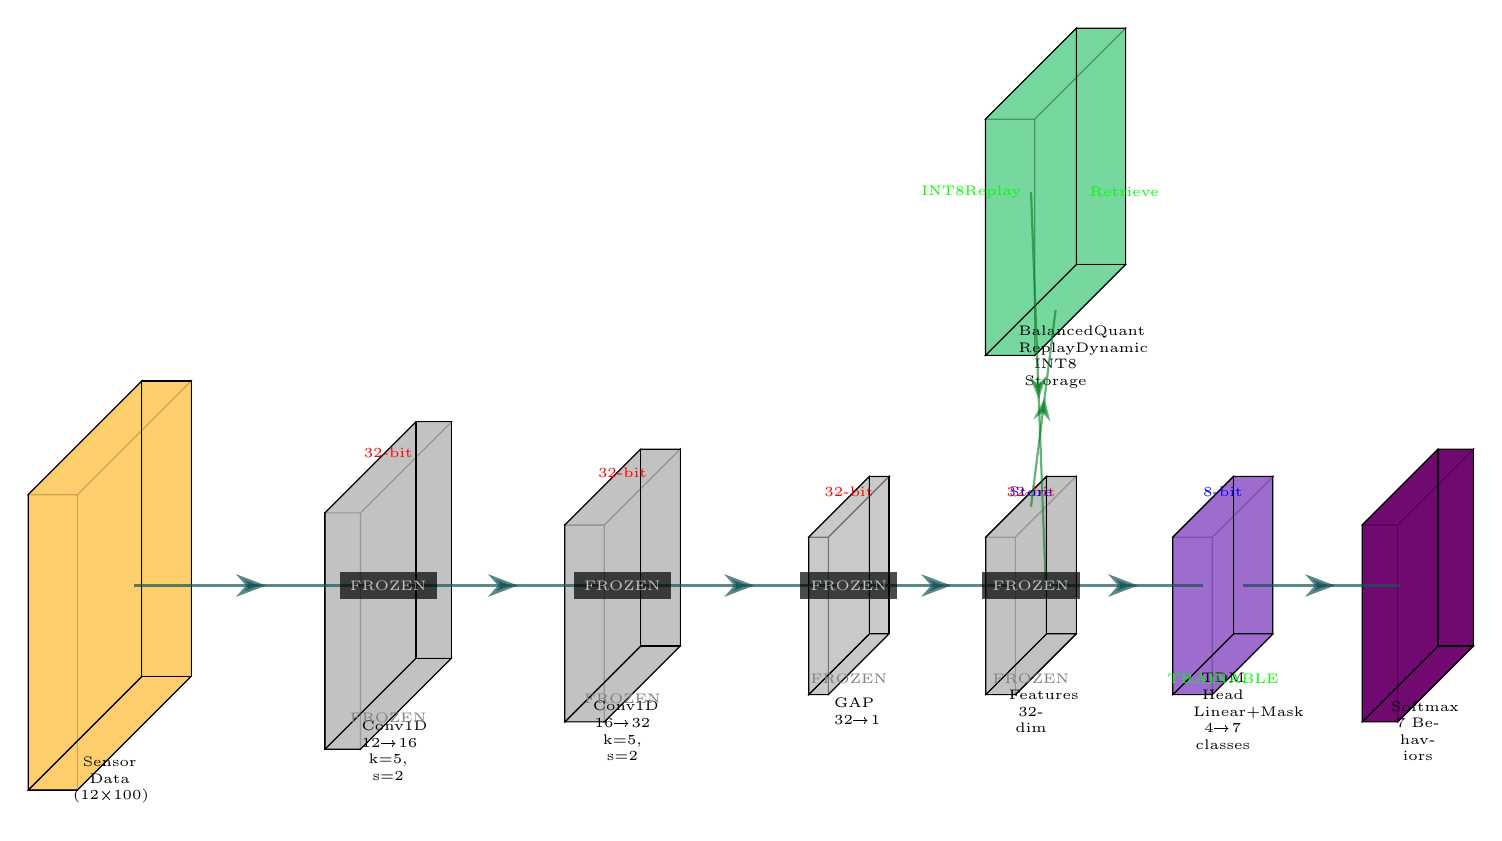
\begin{tikzpicture}[scale=0.7]

%%%%%%%%%%%%%%%%%%%%%%%%%%%%%%%%%%%%%%%%%%%%%%%%%%%%%%%%%%%%%%%%%%%%%%%%%%%%%%%%%%%%%%%%
%% Main CNN Pipeline (horizontal)
%%%%%%%%%%%%%%%%%%%%%%%%%%%%%%%%%%%%%%%%%%%%%%%%%%%%%%%%%%%%%%%%%%%%%%%%%%%%%%%%%%%%%%%%
% Input Layer
\pic[shift={(0,0,0)}] at (0,0,0) {Box={name=input,%
        caption={Sensor Data\\(12×100)},%
        fill=\ConvColor,opacity=0.8,width=2.5,height=15,depth=15,scale=0.25}};

% Conv1D Layer 1 (FROZEN)
\pic[shift={(3,0,0)}] at (input-east) {RightBandedBox={name=conv1,%
        caption={Conv1D\\12→16\\k=5, s=2},%
        fill=\FrozenColor,bandfill=\FrozenColor,opacity=0.8,width=1.8,height=12,depth=12,scale=0.25}};

% Conv1D Layer 2 (FROZEN)
\pic[shift={(2.5,0,0)}] at (conv1-east) {RightBandedBox={name=conv2,%
        caption={Conv1D\\16→32\\k=5, s=2},%
        fill=\FrozenColor,bandfill=\FrozenColor,opacity=0.8,width=2,height=10,depth=10,scale=0.25}};

% Global Average Pooling (FROZEN)
\pic[shift={(2.5,0,0)}] at (conv2-east) {Box={name=gap,%
        caption={GAP\\32→1},%
        fill=\FrozenColor,opacity=0.6,width=1,height=8,depth=8,scale=0.25}};

% Features (FROZEN)
\pic[shift={(2,0,0)}] at (gap-east) {Box={name=features,%
        caption={Features\\32-dim},%
        fill=\FrozenColor,opacity=0.8,width=1.5,height=8,depth=8,scale=0.25}};

% TDM Head (TRAINABLE)
\pic[shift={(2,0,0)}] at (features-east) {Box={name=head,%
        caption={TDM Head\\Linear+Mask\\4→7 classes},%
        fill=\FcColor,opacity=0.8,width=2,height=8,depth=8,scale=0.25}};

% Output
\pic[shift={(2,0,0)}] at (head-east) {Box={name=output,%
        caption={Softmax\\7 Behaviors},%
        fill=\SoftmaxColor,opacity=0.8,width=1.8,height=10,depth=10,scale=0.25}};

%%%%%%%%%%%%%%%%%%%%%%%%%%%%%%%%%%%%%%%%%%%%%%%%%%%%%%%%%%%%%%%%%%%%%%%%%%%%%%%%%%%%%%%%
%% Replay Buffer (above main pipeline)
%%%%%%%%%%%%%%%%%%%%%%%%%%%%%%%%%%%%%%%%%%%%%%%%%%%%%%%%%%%%%%%%%%%%%%%%%%%%%%%%%%%%%%%%
\pic[shift={(0,4,0)}] at (features-north) {Box={name=replay_buffer,%
        caption={BalancedQuant\\ReplayDynamic\\INT8 Storage},%
        fill=\ReplayColor,opacity=0.7,width=2.5,height=12,depth=12,scale=0.25}};

%%%%%%%%%%%%%%%%%%%%%%%%%%%%%%%%%%%%%%%%%%%%%%%%%%%%%%%%%%%%%%%%%%%%%%%%%%%%%%%%%%%%%%%%
%% Main forward connections
%%%%%%%%%%%%%%%%%%%%%%%%%%%%%%%%%%%%%%%%%%%%%%%%%%%%%%%%%%%%%%%%%%%%%%%%%%%%%%%%%%%%%%%%
\draw [connection]  (input-east)    -- node {\midarrow} (conv1-west);
\draw [connection]  (conv1-east)    -- node {\midarrow} (conv2-west);
\draw [connection]  (conv2-east)    -- node {\midarrow} (gap-west);
\draw [connection]  (gap-east)      -- node {\midarrow} (features-west);
\draw [connection]  (features-east) -- node {\midarrow} (head-west);
\draw [connection]  (head-east)     -- node {\midarrow} (output-west);

%%%%%%%%%%%%%%%%%%%%%%%%%%%%%%%%%%%%%%%%%%%%%%%%%%%%%%%%%%%%%%%%%%%%%%%%%%%%%%%%%%%%%%%%
%% Replay buffer connections
%%%%%%%%%%%%%%%%%%%%%%%%%%%%%%%%%%%%%%%%%%%%%%%%%%%%%%%%%%%%%%%%%%%%%%%%%%%%%%%%%%%%%%%%
% From features to replay buffer (storing)
\draw [replayconnection] (features-north) -- node {\replayarrow} (replay_buffer-south);
% From replay buffer to features (retrieving)
\draw [replayconnection] (replay_buffer-west) -- node {\replayarrow} (features-east);

%%%%%%%%%%%%%%%%%%%%%%%%%%%%%%%%%%%%%%%%%%%%%%%%%%%%%%%%%%%%%%%%%%%%%%%%%%%%%%%%%%%%%%%%
%% Precision annotations
%%%%%%%%%%%%%%%%%%%%%%%%%%%%%%%%%%%%%%%%%%%%%%%%%%%%%%%%%%%%%%%%%%%%%%%%%%%%%%%%%%%%%%%%
\node[font=\tiny, color=red] at (conv1-north) [above] {32-bit};
\node[font=\tiny, color=red] at (conv2-north) [above] {32-bit};
\node[font=\tiny, color=red] at (gap-north) [above] {32-bit};
\node[font=\tiny, color=red] at (features-north) [above] {32-bit};
\node[font=\tiny, color=blue] at (head-north) [above] {8-bit};

%%%%%%%%%%%%%%%%%%%%%%%%%%%%%%%%%%%%%%%%%%%%%%%%%%%%%%%%%%%%%%%%%%%%%%%%%%%%%%%%%%%%%%%%
%% Frozen layer annotations
%%%%%%%%%%%%%%%%%%%%%%%%%%%%%%%%%%%%%%%%%%%%%%%%%%%%%%%%%%%%%%%%%%%%%%%%%%%%%%%%%%%%%%%%
\node[font=\tiny, color=gray] at (conv1-south) [below] {FROZEN};
\node[font=\tiny, color=gray] at (conv2-south) [below] {FROZEN};
\node[font=\tiny, color=gray] at (gap-south) [below] {FROZEN};
\node[font=\tiny, color=gray] at (features-south) [below] {FROZEN};
\node[font=\tiny, color=green] at (head-south) [below] {TRAINABLE};

% Add "FROZEN" text overlay on the frozen blocks
\node[font=\tiny, color=white, fill=black, opacity=0.7, text width=1cm, align=center] at (conv1-center) {FROZEN};
\node[font=\tiny, color=white, fill=black, opacity=0.7, text width=1cm, align=center] at (conv2-center) {FROZEN};
\node[font=\tiny, color=white, fill=black, opacity=0.7, text width=1cm, align=center] at (gap-center) {FROZEN};
\node[font=\tiny, color=white, fill=black, opacity=0.7, text width=1cm, align=center] at (features-center) {FROZEN};

%%%%%%%%%%%%%%%%%%%%%%%%%%%%%%%%%%%%%%%%%%%%%%%%%%%%%%%%%%%%%%%%%%%%%%%%%%%%%%%%%%%%%%%%
%% Labels and annotations
%%%%%%%%%%%%%%%%%%%%%%%%%%%%%%%%%%%%%%%%%%%%%%%%%%%%%%%%%%%%%%%%%%%%%%%%%%%%%%%%%%%%%%%%
\node[font=\tiny, color=green] at (replay_buffer-west) [left] {INT8\\Replay};

% Add flow labels
\node[font=\tiny, color=blue] at (features-north) [above] {Store};
\node[font=\tiny, color=green] at (replay_buffer-east) [right] {Retrieve};

%%%%%%%%%%%%%%%%%%%%%%%%%%%%%%%%%%%%%%%%%%%%%%%%%%%%%%%%%%%%%%%%%%%%%%%%%%%%%%%%%%%%%%%%
\end{tikzpicture}
\end{document}
